\documentclass[10pt,a4paper]{article}
\usepackage[margin=19mm]{geometry}
\usepackage[T1]{fontenc}
\usepackage{amsmath,booktabs,graphicx}
\usepackage[hidelinks]{hyperref}
\setlength{\parindent}{0pt}
\setlength{\parskip}{5pt}
\setlength{\emergencystretch}{2em}
\title{\textbf{Explicit Advection in Weather Foundation Models}\\[3pt]\large GraphCast weather, Aurora cyclone tracking, and Aurora air pollution}
\author{Pratyush Kumar Singh (230784)\\[4pt]Supervisor: Prof.\ Rajiv Ratn Shah}
\date{15 November 2026}
\begin{document}
\maketitle
\small
\begin{abstract}
A weather forecast can predict a storm of roughly the right strength and still put it in the wrong place. The same problem comes up with pollution: a plume can look weaker if the forecast spreads it out instead of moving it with the wind. We ask whether giving a forecast model a simple way to move patterns helps it keep their shape and location. We test this idea on short-range weather forecasts, tropical cyclone tracks, and air pollution. The clearest improvement was in cyclone tracking, where one version brought the average three-day position error down by about 18 km. The change in six-hour weather forecasts was very small. Our air-pollution test covered only two forecasts, and errors were often larger than when we simply carried recent concentrations forward. More cases are needed to judge whether the method helps with pollution.
\end{abstract}

\section{Forecasting and transport}
A forecast state \(X_t\) contains surface variables and upper-air fields at fixed pressure levels. Static data \(S\), such as terrain and land--sea mask, describe the grid. A deterministic model uses two recent states and can feed its forecast back as input:
\[
 \begin{aligned}\widehat X_{t+\Delta t}&=F_\theta(X_{t-\Delta t},X_t,S),\\
 \widehat X_{t+2\Delta t}&=F_\theta(X_t,\widehat X_{t+\Delta t},S).\end{aligned}
\]
Fine-tuning adapts released weights to a new grid, data source or task. The autoregressive loss supervises \(K\) forecast times:
\[\mathcal L_K=K^{-1}\sum_{k=1}^K\ell(\widehat X_{t+k\Delta t},X_{t+k\Delta t}).\] \(K\) counts forecast steps within each training window. Optimizer updates count parameter changes.

A simplified advection--diffusion--reaction equation for a scalar \(q\) on the sphere is
\[
 \partial_tq+\boldsymbol u\cdot\nabla_Sq=\kappa\Delta_Sq+s(q,\boldsymbol x,t).
\]
Advection shifts a feature, diffusion spreads gradients, and sources change its amplitude. In one dimension with constant wind, \(q(x,t+\Delta t)=q(x-u\Delta t,t)\). A narrow storm core can move without broadening. A trained model can average uncertain peak locations, motivating an explicit displacement branch. For a surface density, the conservative equation uses \(\nabla_S\cdot(q\boldsymbol u)\), which differs from scalar advection by \(q\nabla_S\cdot\boldsymbol u\).

A backward \emph{pull} estimates the departure point, then interpolates present content there. On the unit sphere, with tangent velocity \(\boldsymbol u\), Earth radius \(R\), and \(\alpha=\|\boldsymbol u\|\Delta t/R\), a frozen-velocity approximation is
\[
 \boldsymbol r_d=\cos\alpha\,\boldsymbol r-\sin\alpha\,\boldsymbol u/\|\boldsymbol u\|.
\]
At zero velocity the point is unchanged. A forward \emph{push} distributes each source into destination cells. If \(A_i\) is source cell area and \(\sum_jw_{ij}=1\), then
\[
 q'_j=A_j^{-1}\sum_i A_iq_iw_{ij},\qquad \sum_j A_jq'_j=\sum_i A_iq_i .
\]
The conservation identity applies to the isolated scatter under complete coverage. Latent features, subsequent mixing, and decoded fields have different physical interpretations.

\newpage
\section{GraphCast weather forecasting}
GraphCast \cite{graphcast} encodes the latitude--longitude grid into a spherical multiresolution mesh, applies graph message passing, and decodes the mesh back to the grid. Message passing aggregates learned interactions over graph edges. The project retains the normal mesh and 37 levels while sampling ERA5 to \(1^\circ\). The native \(0.25^\circ\) inference smoke tests and the 13-level GraphCast-small pilots are separate engineering checks.

The PARADIS-inspired adapter \cite{paradis} acts after the mesh processor. It projects mesh features \(h\) into 16 scalar modes, interpolates them onto a regular grid by inverse-distance weighting, and predicts bounded displacements for each mode. Bicubic sampling uses periodic longitude and pole continuation:
\[
 z=\mathcal I(Ph),\qquad h^+=h+U[\mathcal S(z,\boldsymbol r_d)-\mathcal S(z,\boldsymbol r)].
\]
Subtracting the stationary sample cancels the grid transfer at zero displacement. The lift \(U\) starts at zero, so initially the forecast receives no correction. The offsets describe latent feature motion.

\textbf{Protocol.} Both models trained for 1,000 updates on 2016--2019 ERA5, with batch one, seed 0 and a six-hour horizon. Four fixed 2020 windows select checkpoints. Verification uses 36 monthly dates across 2020--2022. The pretrained checkpoint includes ERA5 through 2017. Normalized validation loss fell from 14.84619 to 0.74184 for direct training and from 14.84814 to 0.74172 with advection.

\textbf{Metrics.} With forecast error \(e_{ij}\) at date \(i\) and cell \(j\), and area weight \(a_j\),
\[
 \mathrm{RMSE}=\sqrt{\frac{\sum_{ij}a_j e_{ij}^2}{\sum_{ij}a_j}},\qquad
 \mathrm{ACC}_i=\frac{\sum_j a_j f'_j y'_j}{\sqrt{\sum_j a_j(f'_j)^2\sum_j a_j(y'_j)^2}}.
\]
ACC averages date scores after removing the 1990--2019 ERA5 climatology. ACC covers supported levels and surface fields. RMSE covers all 37 levels.

\begin{center}
\textbf{Combined 2021--2022 test at +6 h}\\[3pt]
\begin{tabular}{@{}llrrrr@{}}
\toprule Field & Unit & Direct RMSE & Adv.\ RMSE & Direct ACC & Adv.\ ACC\\\midrule
2 m temperature & K & .59500 & .59485 & .974273 & .974285\\
850 hPa temperature & K & .33982 & .33987 & .995269 & .995269\\
500 hPa geopotential & m$^2$/s$^2$ & 22.79157 & 22.78831 & .999600 & .999601\\
10 m east wind & m/s & .48596 & .48587 & .992172 & .992175\\
10 m north wind & m/s & .49700 & .49655 & .992437 & .992451\\
Sea-level pressure & Pa & 32.44268 & 32.45245 & .998948 & .998948\\
6 h precipitation & mm & 1.09497 & 1.09506 & .881912 & .881923\\\bottomrule
\end{tabular}
\end{center}
On the separate 12-date 2020 diagnostic, 2 m RMSE is 2.239944 K pretrained, 0.583608 K after direct fine-tuning, 0.583768 K with trained advection, and 0.583783 K with its correction disabled. The on/off gap of 0.000015 K is below the observed repeat standard deviations of 0.000057--0.000072 K on a fixed date. Mean sampling distance rises from 215.39 to 263.08 km equivalent, and changing only displacement weights with backbone features fixed changes offsets by 6.64\% in relative \(L^2\). Correction RMS is 0.13411\% of backbone feature RMS. The learned geometry is measurable, while these tests establish little incremental forecast benefit. \href{https://github.com/Xavaitron/Weather_foundational_model/tree/e348e2a/graphcast-weather/results}{Yearly tables, level-wise scores and ablations.}

\newpage
\section{Aurora cyclone tracking}
Aurora \cite{aurora} encodes fields and levels with a Perceiver-style encoder, evolves features with a 3D Swin Transformer, and decodes physical forecasts. The original pretrained Aurora uses a \(120\times240\), \(1.5^\circ\) weather grid here. Its \(4\times4\) patches give a \(30\times60\) transport lattice. Aurora 1.5 is a separate model name.

The transport branch encodes current dynamic fields, estimates grouped horizontal motion using recent history and backbone context, and corrects features before decoding. For current features \(c_t\), backbone forecast \(b\), projection \(P\), lift \(U\) and small learned gain \(g\),
\[
 \widetilde c=\mathcal T(c_t,\boldsymbol u)+\mathcal R,\qquad
 b^+=b+\tanh(g)\,U(\widetilde c-Pb),\qquad\widehat X=D(b^+).
\]
The slot features are learned scalars. As the gain goes to zero the forecast recovers the standard decoder path.

\begin{description}
\item[Standard.] Fine-tunes the original encoder, backbone and decoder with normalized variable-weighted weather MAE.
\item[PARADIS-inspired.] Pulls features at spherical departure points with bicubic interpolation and adds depthwise mixing and pointwise reaction/source updates \cite{paradis}.
\item[NowcastNet-inspired.] Uses nearest-neighbour backward transport plus a learned source \cite{nowcast}. Nearest sampling has zero coordinate derivatives almost everywhere. A second bilinear forecast supplies gradients, with objective \(\ell_{\rm near}+0.5\ell_{\rm bilinear}\). Inference uses the nearest branch.
\item[ADRNet-inspired.] Uses area-weighted forward splatting, local reaction and implicit diffusion \cite{adr}. The diffusion solves \((I-\eta L_{\rm grid})c_{\rm diff}=c_{\rm push}\); each eigenmode of \(-L_{\rm grid}\) with eigenvalue \(\lambda\ge0\) is scaled by \(1/(1+\eta\lambda)\). Longitude is periodic and latitude uses Neumann boundaries.
\item[de B\'ezenac-inspired.] Learns a departure point and positive width \(\sigma\) for a normalized \(7\times7\) Gaussian pull \cite{bezenac}:
\[
 w_i=\frac{\exp[-\|\boldsymbol x_i-\boldsymbol x_d\|^2/(2\sigma^2)]}
 {\sum_j\exp[-\|\boldsymbol x_j-\boldsymbol x_d\|^2/(2\sigma^2)]}.
\]
\end{description}

\textbf{Data and optimization.} WeatherBench 2 HRES-T0 provides six-hour atmospheric states and targets, with ERA5 static fields. NOAA IBTrACS provides verifying storm positions \cite{wb,ibtracs}. Training uses 2016--2020, validation 2021, and test 2022. All five models use 10,000 AdamW updates, seed 42, BF16, checkpointing, and four microbatches of one per update. Two-step training supervises +6 and +12 h with gradients through both. A four-step setup extends this to +24 h. Its results are pending. Best checkpoints minimize validation weather loss. The NowcastNet auxiliary objective differs from the other variants.

\textbf{Tracker and scores.} The tracker starts from a known storm, searches forecast sea-level pressure and 700 hPa geopotential for a centre, and refines below grid spacing. A failure persists the previous predicted location and stays in the scores. The distance for predicted and observed coordinates is
\[
 d=2R\arcsin\sqrt{\sin^2[(\widehat\varphi-\varphi)/2]
 +\cos\widehat\varphi\cos\varphi\sin^2[(\widehat\lambda-\lambda)/2]} .
\]
Track MAE averages \(d\); RMSE is \(\sqrt{\operatorname{mean}(d^2)}\), which emphasizes large misses. The paired bootstrap samples 1,000 storm clusters within basins. Intervals are nominal and pointwise. Results use zero issue delay.

\newpage
\subsection{Cyclone results}
\begin{center}
\begin{tabular}{@{}lrrrrr@{}}
\toprule Global track MAE (km) & 24 h & 48 h & 72 h & 96 h & 120 h\\\midrule
Standard & 209.67 & 325.86 & 468.82 & 585.35 & 720.98\\
PARADIS & 207.99 & 319.74 & 464.01 & 569.27 & 723.54\\
NowcastNet & 204.84 & 319.58 & 450.43 & 568.65 & 714.10\\
ADRNet & 205.77 & 321.28 & 462.35 & 575.90 & 719.57\\
de B\'ezenac & 207.93 & 321.78 & 463.30 & 579.32 & 722.02\\
\midrule Cases & 2109 & 1699 & 1329 & 1024 & 780\\
Distinct storms & 109 & 102 & 91 & 80 & 62\\\bottomrule
\end{tabular}

\smallskip
\begin{tabular}{@{}lrrrrr@{}}
\toprule Global track RMSE (km) & 24 h & 48 h & 72 h & 96 h & 120 h\\\midrule
Standard & 289.45 & 452.84 & 661.80 & 821.99 & 985.54\\
PARADIS & 287.97 & 440.79 & 651.76 & 803.64 & 1001.79\\
NowcastNet & 281.26 & 446.23 & 632.20 & 798.04 & 978.37\\
ADRNet & 280.81 & 444.37 & 638.65 & 792.84 & 974.34\\
de B\'ezenac & 284.02 & 445.80 & 648.66 & 808.48 & 976.58\\\bottomrule
\end{tabular}
\end{center}
NowcastNet gives the lowest global MAE at each lead. At 72 h the relative change is \(-3.92\%\) with a nominal interval of \([-6.73,-1.46]\%\). The model improves mean error for 56 of 91 storms at this lead. Nominal paired intervals favor NowcastNet on days 1, 3 and 4, PARADIS on days 2 and 4, and ADRNet on day 1. Every day-five interval includes zero. ADRNet leads the RMSE table on days 1, 4 and 5. Day-five tracker failures are 10.77\% for standard and 11.41--12.05\% across the adapters. The study uses one seed and one test year.

\begin{center}
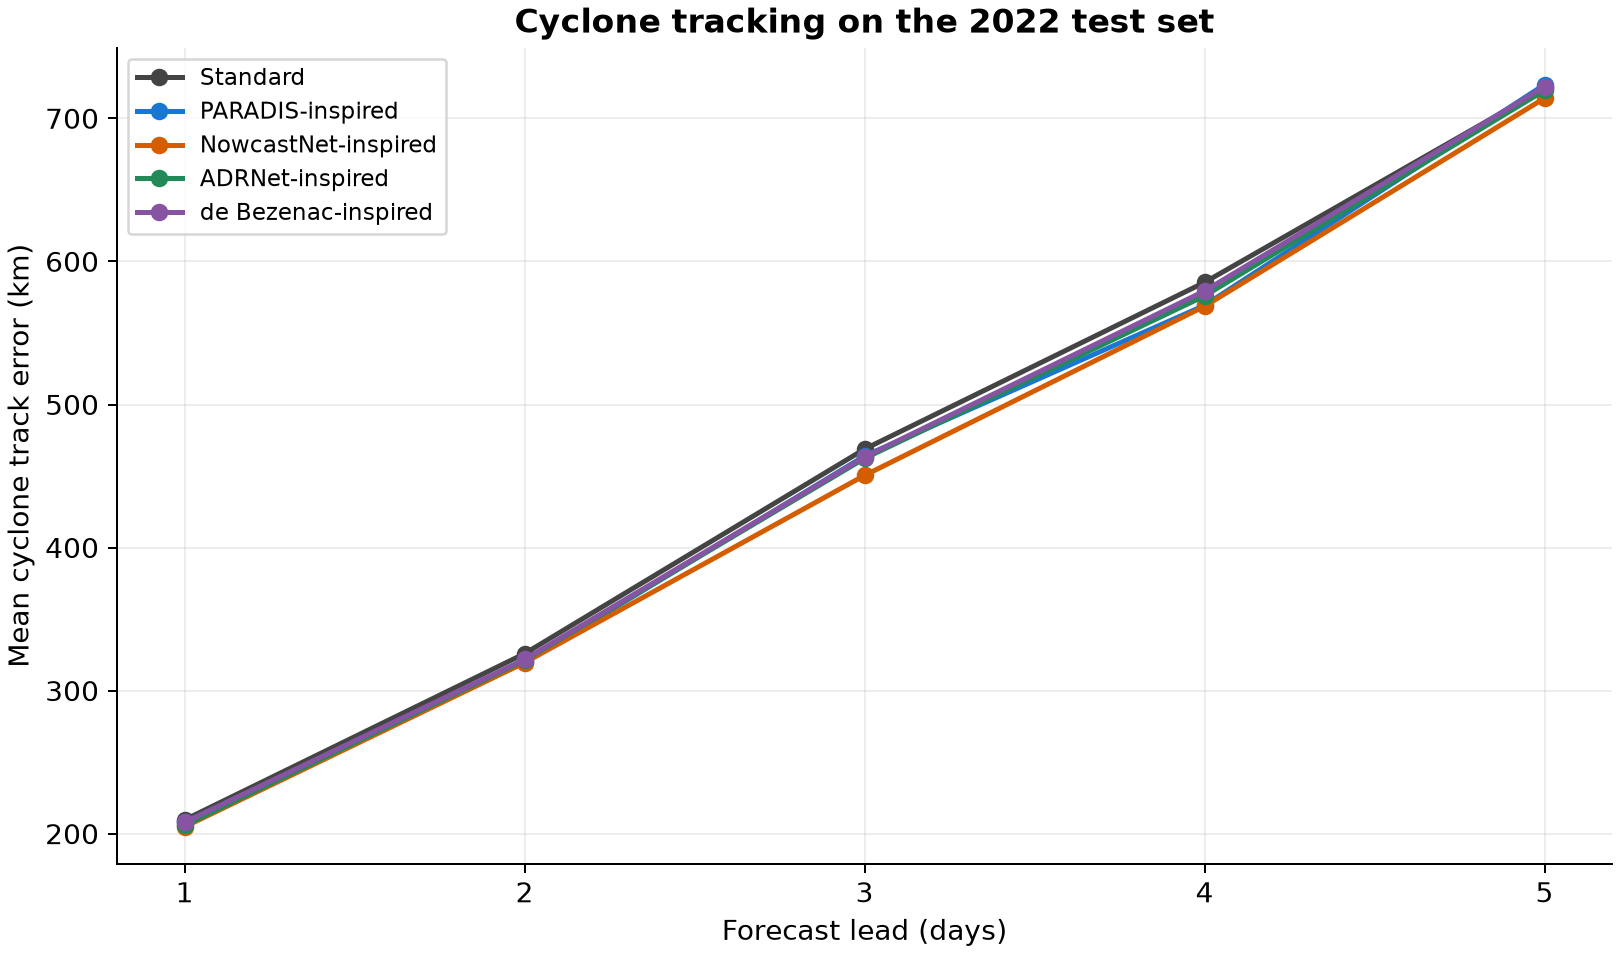
\includegraphics[width=.63\linewidth,height=.25\textheight,keepaspectratio]{figures/track_error_by_lead.png}\\[-2pt]
\textit{Global MAE rises with lead across all five models.}
\end{center}
Best normalized validation losses range from 0.043832 (NowcastNet) to 0.044086 (standard). Median update time is 6.82 s for NowcastNet and 4.76 s for standard. Peak PyTorch allocation is 27.46 and 26.19 GiB, respectively. \href{https://github.com/Xavaitron/Weather_foundational_model/tree/e348e2a/aurora-cyclone-tracking/results}{Full failure rates, basin intervals and training costs.}

\textbf{Published \(0.25^\circ\) reference.} Bodnar et al.\ report about 6\% lower track MAE at day 1 and 20--25\% at days 2--5 versus official forecasts in North Atlantic and East Pacific examples \cite{aurora}. Their HRES-T0 Aurora evaluation spans 2022--2023 with different comparators, timing and cases. A native-resolution run on the same local 2022 cases remains pending.

\newpage
\section{Aurora air pollution}
The project extends the official 12-hour Aurora \emph{weather} checkpoint with pollutant inputs and outputs. At \(1.5^\circ\) it predicts 142 channels, including 73 pollutant channels. Horizontal transport moves plumes; emissions, chemistry, deposition and vertical mixing alter concentrations. The learned branch uses wind and pollutant history to correct the decoded pollutant field:
\[
 \widehat q=F_\theta(X)_{\rm pollution}
 +s_{\rm train}C_\phi(q_{\rm history}/s_{\rm train},\Delta\boldsymbol r_{\rm wind}).
\]
The wind proxy uses 10 m wind for surface PM, same-level wind for upper-air species and pressure-thickness weighted wind for total columns. Wind is frozen over the 12-hour displacement interval.

\begin{center}
\begin{tabular}{@{}lp{.70\linewidth}@{}}
\toprule Variant & Correction\\\midrule
Baseline & Full fine-tuning with the expanded Aurora outputs.\\
Fixed wind pull & Adds the difference between wind-transported and current fields.\\
Column push & Scatters area-weighted content for five total columns.\\
NowcastNet & A two-resolution U-Net predicts motion residuals and an additive source.\\
ADRNet & Three reaction, bounded explicit diffusion and pull blocks on 32 latent channels.\\
de B\'ezenac & A U-Net predicts motion for a normalized \(6\times6\) Gaussian pull.\\\bottomrule
\end{tabular}
\end{center}
The loss averages area-weighted MAE across channels after dividing by each channel's training-period persistence MAE. Held-out scoring records RMSE, MAE, signed bias, and the area fraction below zero. Fixed persistence repeats the last field. Diurnal persistence repeats the last field at the same time of day.

\textbf{January EAC4 pilot.} Train 1--20 January 2003 (38 windows), validate 21--24 January (6 windows), and test 25--31 January. With seed 42 the baseline completes 200 updates and validation loss reaches 1.8197 from 2.8825 at step 50. Two overlapping starts, 25 and 26 January at 12 UTC, support ten forecast steps to +120 h. EAC4 reanalysis supplies the reference; the India region is a geographic bounding box.

\begin{center}
\begin{tabular}{@{}llrrrr@{}}
\toprule Region & Lead & Aurora RMSE & Fixed persist. & Diurnal persist. & Negative area\\\midrule
Global & 12 h & 24.251 & 17.207 & 18.828 & 15.52\%\\
Global & 24 h & 24.595 & 19.555 & 19.555 & 17.96\%\\
Global & 72 h & 26.026 & 24.599 & 24.599 & 20.20\%\\
Global & 120 h & 20.888 & 22.530 & 22.530 & 19.74\%\\
India & 12 h & 50.785 & 38.981 & 19.199 & 5.07\%\\
India & 24 h & 30.950 & 13.293 & 13.293 & 8.72\%\\
India & 72 h & 24.710 & 20.193 & 20.193 & 8.21\%\\
India & 120 h & 25.933 & 21.321 & 21.321 & 7.98\%\\\bottomrule
\end{tabular}\\
\textit{PM2.5 RMSE in micrograms per cubic metre. Negative area uses raw predictions.}
\end{center}
India PM2.5 trails both persistence controls at all reported leads. The global day-five score beats persistence for these two cases. All variants passed two EAC4 integration updates, while matched held-out adapter scores remain pending. The archived historical EAC4 download reached January 2013 before an ADS TLS failure. The full all-pollutant evaluation JSON is absent from the repo. Published Aurora at \(0.4^\circ\) beats its chemistry comparator on 74\% of evaluated targets \cite{aurora}; the January pilot uses the weather checkpoint and cannot supply a local \(0.4^\circ\) score.

\newpage
\section{Diagnostics and interpretation}
\begin{center}
\begin{tabular}{@{}lrrrrr@{}}
\toprule Cyclone tracker failure & 24 h & 48 h & 72 h & 96 h & 120 h\\\midrule
Standard & 5.22\% & 8.06\% & 9.86\% & 10.25\% & 10.77\%\\
PARADIS & 5.36\% & 8.06\% & 9.10\% & 10.55\% & 11.41\%\\
NowcastNet & 4.88\% & 7.00\% & 9.18\% & 9.47\% & 11.41\%\\
ADRNet & 5.17\% & 7.65\% & 9.18\% & 10.25\% & 12.05\%\\
de B\'ezenac & 5.36\% & 7.95\% & 9.71\% & 10.06\% & 11.67\%\\\bottomrule
\end{tabular}

\medskip
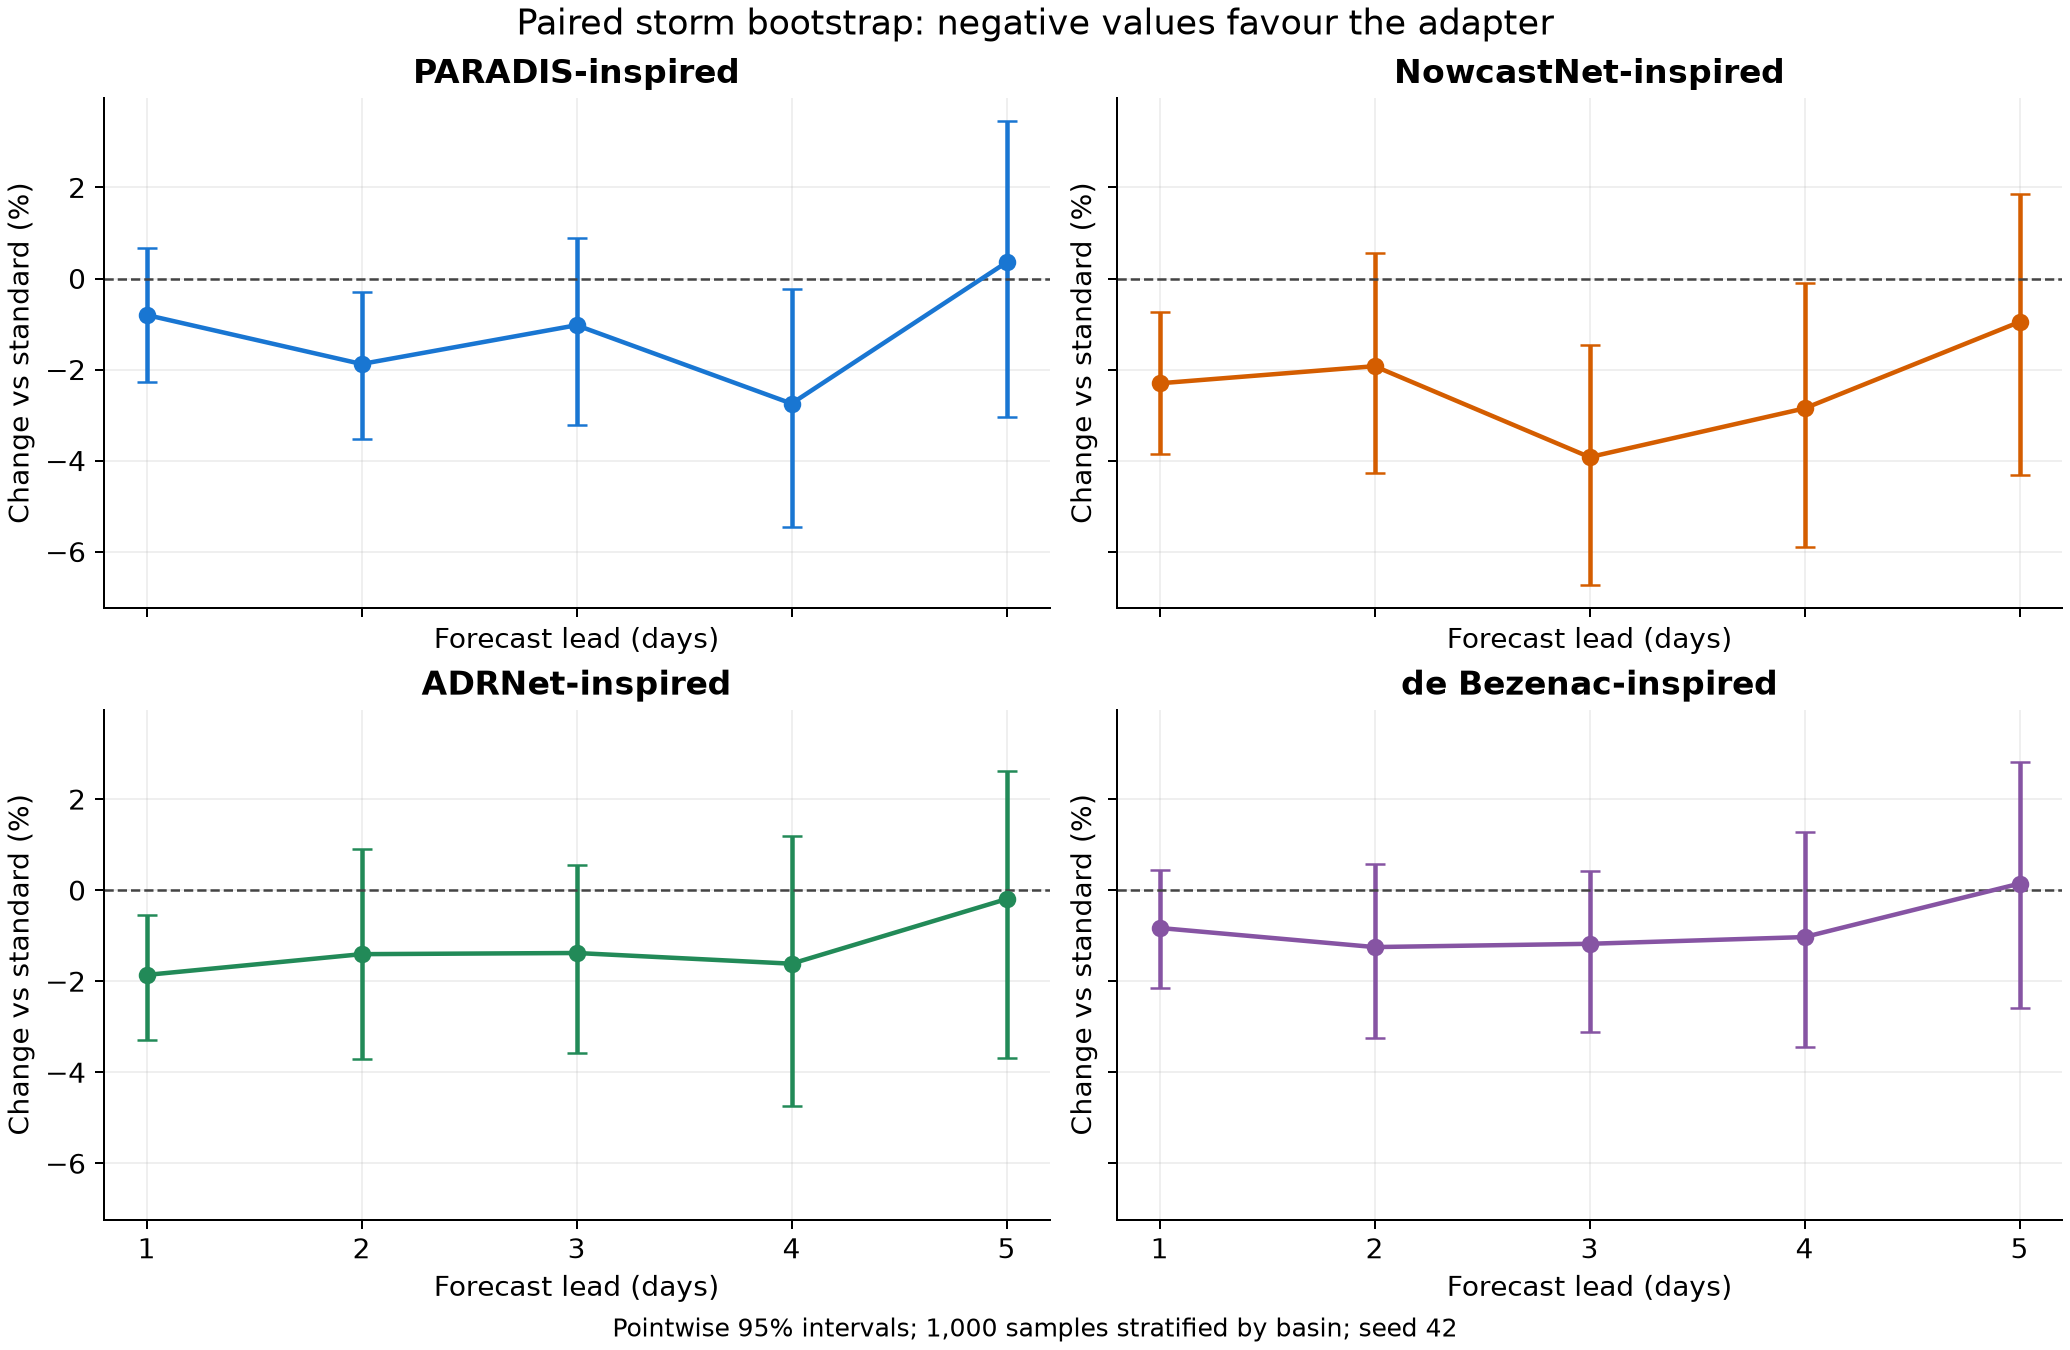
\includegraphics[width=.84\linewidth,height=.32\textheight,keepaspectratio]{figures/relative_error_confidence_intervals.png}\\
\textit{Paired change in cyclone MAE. Horizontal error bars show nominal 95\% intervals.}
\end{center}
GraphCast measures global weather fields and can be insensitive to small changes confined to a moving region. Cyclone verification measures position for initialized storms, with fewer cases at long leads. The day-three improvement does not isolate transport from the additional NowcastNet auxiliary loss. Regional results vary and can rely on small storm counts. Pollution verification measures concentration and needs stronger persistence and seasonal comparisons, along with checks for negative predictions.

\textbf{Engineering scope.} GraphCast compiler memory estimates for one update were 10.77 GiB for full-model \(1^\circ\) standard training and 10.98 GiB with advection. The \(0.1^\circ\) profiles exceeded the tested GPU capacity. Cyclone memory numbers are measured PyTorch allocations and should not be directly compared to XLA estimates. The real-data pollution baseline trial allocated about 23.50 GiB. Engineering trials establish that an update runs under a specific setup.

\textbf{Complete numerical evidence.}
The \href{https://github.com/Xavaitron/Weather_foundational_model/tree/e348e2a}{source snapshot} contains the year-by-year GraphCast tables and full variable/level CSV, the cyclone global and 140 paired comparisons including basin intervals, and the dated air-pollution results. It also documents setup, evaluation commands and data splits. The linked workflow results also include exact values and additional plots.

\newpage
\section{The Mathematics Behind the Transport Operators}
Let \(c_{ij}\) be the current feature at grid cell \((i,j)\). To make a pull forecast at a destination, we first use the learned motion to find a departure point. Suppose that point lies between four cells at fractions \(a,b\in[0,1]\). Bilinear interpolation gives
\[
 B(c;a,b)=(1-a)(1-b)c_{00}+a(1-b)c_{10}+(1-a)bc_{01}+ab c_{11}.
\]
For example, \(a=0.25\) and \(b=0\) give \(0.75c_{00}+0.25c_{10}\). Along that edge, the result changes with \(a\) at rate \(c_{10}-c_{00}\). This lets the forecast loss teach the model where to sample.

\paragraph{PARADIS: move, mix, and add.}
The cyclone variant first computes \(v=\operatorname{Bicubic}(c,\boldsymbol r_d)\). Bicubic sampling uses four points in each direction. It then applies
\(c^+=v+M(v)+R(v)+s\) for one substep. \(M\) mixes nearby cells within each channel. \(R\) mixes channels at the same cell. The learned source \(s\) adds local changes. The GraphCast variant borrows the bicubic move and uses the difference between displaced and stationary samples as its correction.

\paragraph{NowcastNet: move and add a source.}
The cyclone branch predicts \(c^+_{\rm near}=N(c,\boldsymbol r_d)+s\), where \(N\) picks the nearest cell. Moving the sample a little usually leaves that cell unchanged, so its coordinate gradient is zero. Training also predicts \(c^+_{\rm bil}=B(c,\boldsymbol r_d)+s\). Both branches use the same motion and source. The extra bilinear loss trains the motion. The pollution variant instead adds a gated bilinear change \(g[B(q,\boldsymbol r_d)-q]\) and a learned source to the decoded pollutant forecast.

\paragraph{ADRNet: transport, diffuse, and react.}
The cyclone variant scatters source cells forward and divides by destination area. Diffusion solves \((I-\eta L)c_{\rm diff}=c_{\rm push}\), then the source is added. In the five-point grid stencil, \(Lc=\sum_{\rm four\ neighbors}c_j-4c\). The implicit solve reduces fine-scale variation. The pollution variant uses a different order: a local reaction, an explicit diffusion step \(c^+=c+\eta Lc\), and a bilinear pull. In that diffusion step, the centre gets weight \(1-4\eta\) and each neighbour gets weight \(\eta\). With \(0<\eta<1/4\), all five weights are positive and sum to one.

\paragraph{de B\'ezenac: Gaussian sampling.}
This variant computes \(\sum_i w_i c_i\), with the normalized Gaussian weights from Section~3. A small width \(\sigma\) gives more weight to cells close to the departure point. A larger width spreads the weight across more cells and smooths the result. The cyclone and pollution variants use \(7\times7\) and \(6\times6\) sampling windows, respectively. Since the weights sum to one, a constant field stays constant. That property does not guarantee that the sum of a density over the globe stays fixed.


\begin{thebibliography}{9}
\bibitem{graphcast} R. Lam et al., Learning skillful medium-range global weather forecasting, \emph{Science}, 2023. \href{https://doi.org/10.1126/science.adi2336}{DOI}.
\bibitem{aurora} C. Bodnar et al., A foundation model for the Earth system, \emph{Nature}, 2025. \href{https://doi.org/10.1038/s41586-025-09005-y}{DOI}.
\bibitem{paradis} C. A. Pereira et al., Learning to Advect: A Neural Semi-Lagrangian Architecture for Weather Forecasting, 2026. \href{https://arxiv.org/abs/2601.21151}{arXiv}.
\bibitem{nowcast} Y. Zhang et al., Skilful nowcasting of extreme precipitation with NowcastNet, \emph{Nature}, 2023. \href{https://doi.org/10.1038/s41586-023-06184-4}{DOI}.
\bibitem{adr} N. Zakariaei et al., Advection Augmented Convolutional Neural Networks, 2024. \href{https://arxiv.org/abs/2406.19253}{arXiv}.
\bibitem{bezenac} E. de B\'ezenac, A. Pajot and P. Gallinari, Deep Learning for Physical Processes, 2017. \href{https://arxiv.org/abs/1711.07970}{arXiv}.
\bibitem{wb} S. Rasp et al., WeatherBench 2, 2024. \href{https://doi.org/10.1029/2023MS004019}{DOI}.
\bibitem{ibtracs} NOAA NCEI, International Best Track Archive for Climate Stewardship (IBTrACS), v04r01. \href{https://www.ncei.noaa.gov/products/international-best-track-archive}{Dataset}.
\end{thebibliography}
\end{document}
